\chapter{Résumé}

\minitoc[n] % minitoc without title

\section{Introduction}

	\subsection{La Coopération} % TODO: changer

		La coopération est un comportement qui se retrouve à toutes les strates de complexité du monde animal. Ses différentes formes sont variées et sont parfois centrales dans de nombreuses espèces. Strictement, la coopération est défini comme un comportement où un acteur (c'est-à-dire l'individu initiant la coopération) agit d'une manière qui est bénéfique à un destinataire~\parencite{West2007a}. Cette définition couvre un large éventail d'actions collectives.

		Comme expliqué précédemment, on peut trouver des exemples de coopération à presque tous les niveaux de complexité du vivant. Par exemple, des êtres unicellulaires tels que les bactéries sont connues pour fréquemment se comporter de manière coopérative. Ces organismes utilisent notamment des sécrétions afin de pouvoir partager des ressources et communiquer~\parencite{Elena2003}. Nous pouvons citer l'exemple particulier des \emph{Pseudomonas aeruginosas} qui sont capable de produire des nutriments que tout organisme voisin peut utiliser. Mais ce qui est particulièrement intéressant dans cet exemple est que produire ces nutriments est coûteux pour ces organismes. Ceci crée une situation complexe connue en biologie ainsi qu'en économie comme de \emph{public goods games}~\parencite{Popat2012, Harrison2013}, que nous pourrions grossièrement traduire par \emph{dilemme des biens publics}. L'idée importante derrière ce terme est que ce genre d'acte de coopération est sensible à l'exploitation par des tricheurs. Ce terme ne traduit pas de jugement moral sur les comportements de ces individus mais permet simplement de transmettre l'idée que ces individus profitent des nutriments d'autres individus sans eux-mêmes participer. C'est-à-dire qu'ils profitent des bénéfices de la coopération sans avoir à en payer le coût.

	  \begin{figure}[hbt]
	      \begin{center}
	        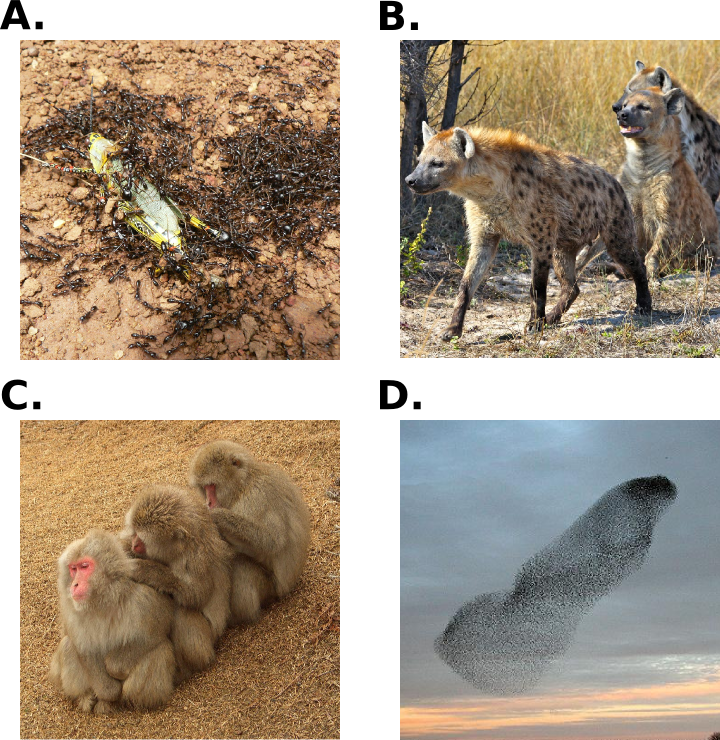
\includegraphics[scale = 0.5]{fig/Intro/CooperationExamples.png}
	        \caption{\textbf{La coopération à différents niveaux de complexité.} {\em (A)}~Les insectes eusociaux (comme les fourmis) possèdent une structure sociale extrêmement avancée. {\em (B)}~Les carnivores sociaux sont capables de coopération avancée ainsi que de se coordonner durant des chasses collectives. {\em (C)}~Le toilettage social est une activité durant laquelle les individus se toilettent à tour de rôle. {\em (D)}~Les volées d'oiseaux montrent l'émergence de déplacements collectifs d'une manière qui laisserait penser que les individus ne font partie que d'une seule entité.} 
	        \label{fig:CooperationExamples}
	      \end{center}
	  \end{figure}

		Un autre célèbre exemple de coopération est celui des insectes \emph{eusociaux}~\parencite{Wilson1990} (voir Figure~\ref{fig:CooperationExamples}~(A)). L'eusocialité est une forme extrême de société qui se retrouvent principalement chez les Hymenoptère (par exemple les fourmis, guêpes et abeilles) et Isoptère (notamment les termites). L'eusocialité est définie par des exemples avancés de coopération. En particulier, le soin des jeunes est pris en charge de manière collective par d'autres individus qui ne sont pas leur parents. Les animaux eusociaux font aussi généralement preuve d'une forme avancée de division du travail, où les individus se partagent une tâche en se répartissant en plusieurs rôles. Enfin, et c'est une des caractéristiques principales de l'eusocialité, il y a aussi une division de la reproduction. Ceci veut dire qu'il existe des castes reproductives et non-reproductives.

		Si nous dézoomons encore le niveau auquel nous observons le monde animal, nous pouvons nous intéresser aux comportements coopératifs des vertébrés. En particulier, les carnivores sociaux sont capables d'actions collectives poussées. Ces espèces sont notamment souvent connues pour leurs comportements de chasse collective où plusieurs individus sont capables de se coordonner afin d'attraper ensemble une proie qu'un individu seul n'aurait pu chasser. Les hyènes tâchetées (Figure~\ref{fig:CooperationExamples}~(B)) par exemple usent de signaux de communication avancés afin d'être capable de pouvoir chasser ensemble. Mais elles vivent aussi dans des groupes sociaux très organisés où les femelles sont en haut de la hiérarchie. Les femelles dominantes sont généralement les seules à se reproduire tandis que les femelles de rang inférieur s'occupent du soin des jeunes des dominantes. Nous pouvons aussi faire référence aux primates, qui ont des structures sociales très fortes. Ces derniers s'engagent notamment dans des du toilettage mutuel (voir Figure~\ref{fig:CooperationExamples}~(C)) entre différents individus du groupe.

		Enfin, à un niveau encore supérieur, nous pouvons citer les comportements de déplacement collectifs, par exemple des volées d'oiseaux (Figure~\ref{fig:CooperationExamples}~(D)). De manière, de nombreux animaux différents peuvent s'organiser en volée, troupeau ou bancs d'individus~\parencite{Couzin2002, Counzin2003}. Ces comportements d'agrégation ont de nombreux avantages pour le group tels qu'augmenter la confusion d'un prédateur, diminuer le risque d'un individu en particulier d'être attaqué ou se défendre de manière collective.


	\subsection{L'Évolution de la Coopération}

		Malgré l'omniprésence de la coopération dans le monde animal, expliquer son évolution est un des défi majeur en biologie évolutionniste.~\parencite{Hamilton1964, Dugatkin2002, West2011a}. En effet le principe de l'évolution tel que théorisé par Darwin peut être résumé par l'expression de la "survie du plus apte"~\parencite{Darwin1859}. Par conséquent, le comportement d'un individu ne peut être adaptatif que s'il lui est bénéfique. Plus précisément, le matériel génétique d'un individu se transmet lors de la reproduction. De là il ressort que, pour qu'un gène puisse se transmettre et donc se répandre dans la population, il est nécessaire qu'il permette à l'individu qui le possède d'augmenter sa capacité reproductive. Un trait particulier n'est donc adaptatif que s'il permet d'augmenter le nombre de descendants d'un individu (ce qu'on appelle valeur sélective).

		C'est sur ce point que l'évolution de la coopération semble être une contradiction. En effet, par définition, un comportement coopératif apporte un bénéfice à un autre individu. A partir de maintenant, lorsque nous ferons mention de bénéfices et coûts, nous nous référerons aux bénéfices et coûts à la valeur sélective des individus. C'est-à-dire que, lorsqu'un comportement est bénéfique à un individu, c'est qu'il permet \emph{au final} à cet individu d'accroître son nombre de descendants. Un comportement coopératif est donc un comportement qui augmente la valeur sélective d'un autre individu. Parfois même, coopérer est coûteux (d'un point de vue de la valeur sélective donc) pour l'acteur. C'est par exemple le cas pour notre exemple précédent des \emph{P. aeruginosas}, pour qui sécréter des nutriments est coûteux. Cet exemple peut nous servir à mieux illuster le problème posé par l'évolution de la coopération. Imaginons une situation où des organismes coopèrent et sécrètent donc des nutriments qui peuvent être utilisés par tous. Imaginons maintenant qu'un mutant apparaît aléatoirement dans cette population et que ce mutant possède un trait qui le pousse à tricher plutôt que coopérer. Il va donc profiter des nutriments sécrétés par les coopérateurs sans lui-même produire ces nutriments et donc en payer le coût. Par conséquent, sa valeur sélective sera supérieure à celle des coopérateurs. Il va donc pouvoir produire plus de descendants et son génotype de tricheur va pouvoir se répandre dans la population. Ceci va continuer jusqu'à que la population ne soit plus composée que de tricheurs. Il apparaît donc que la coopération ne devrait pas être stable. De nombreux modèles ont donc été proposés afin de définir des mécanismes pour expliquer l'évolution de la coopération. Ces mécanismes peuvent être majoritairement classés en deux catégories: les bénéfices \emph{directes} ou \emph{indirectes} à la valeur sélective~\parencite{West2007a}.

		Les bénéfices indirectes permettent notamment d'expliquer l'évolution de \emph{l'altruisme}. L'altruisme est un cas particulier de coopération dont nous avons précédemment parlé où coopérer est coûteux pour l'acteur du comportement coopératif~\parencite{Hamilton1964, West2007a}. Le comportement des \emph{P. aeruginosas} peut en effet être considéré comme altruiste. La division de la reproduction chez les insectes eusociaux, où seule une certaine caste d'individus peut avoir des descendants est aussi un exemple d'altruisme. Les individus non-reproducteurs paient en effect le coût maximal puisqu'ils ne possèdent pas de descendants du tout et ne peuvent donc pas transmettre leur matériel génétique. Il est donc difficile de comprendre comment un tel comportement peut être stable. Le mécanisme permettant d'expliquer l'évolution de l'altruisme a été proposé par Hamilton et s'appelle la \emph{sélection de parentèle}~\parencite{Hamilton1964}. Derrière ce terme est l'idée qu'un trait peut être transmis à travers les parents d'un individu. Si on considère en effet que l'unité de sélection est le gène, c'est-à-dire que l'évolution est due au fait qu'un gène permettant à un individu d'augmenter son nombre de descendants pourra ainsi se répandre dans la population, il n'est pas nécessaire que l'individu possédant ce gène se reproduise. En effet, s'il permet d'aider un individu qui est génétiquement proche de lui (un parent donc), il peut ainsi permettre à un gène permettant un comportement altruiste de se répandre aussi. La valeur sélective d'un trait n'est donc pas dépendante uniquement de la valeur sélective de l'individu possédant ce trait, mais aussi de celle de ces parents. C'est ce qu'on appelle la \emph{valeur sélective inclusive}. Ainsi un trait peut apporter des bénéfices indirectes en augmentant cette valeur sélective inclusive.

		Mais, tandis qu'un très grand nombre de travaux a été concentré sur l'évolution de l'altruisme et les bénéfices indirectes, la plupart des comportements coopératifs bénéficient directement à l'acteur. Dans ce cas, et l'acteur et le destinataire bénéficient du comportement coopératif. On parle aussi de comportement mutuellement bénéfiques pour cette catégorie de la coopération~\parencite{Bergmuller2007a}. Plusieurs mécanismes peuvent permettre d'expliquer comment la coopération peut-être adaptative grâce à des bénéfices directes. En particulier, ces bénéfices peuvent être forcés à travers de la réciprocité, des punitions ou encore des récompenses. Mais ces bénéfices peuvent aussi ne pas être forcés dans le cas où tous les individus partagent un intérêt à coopérer. Dans ce cas, on parle aussi parfois de \emph{bénéfices dérivés} afin de transmettre l'idée que la coopération peut-être dérivé d'un acte originellement égoïste. par exemple, faire partie d'un groupe plus grand d'individus permet d'augmenter les chances de survie (aussi bien face à l'environnement que contre des prédateurs) mais permet aussi de tirer des bénéfices plus importants de la chasse et de la récolte~\parencite{Clutton-Brock2002}. Une partie de la littérature sur la coopération mutuellement bénéfique s'intéresse aussi la coopération entre individus d'espèces différentes, ou coopération inter-espèces. Ceci s'appelle aussi du mutualisme (créant parfois une confusion avec le concept plus général de comportement mutuellement bénéfique). Par exemple, une certaine espèce de poissons, les Labres, sont connus pour le fait qu'ils nettoient d'autres poissons plus gros de leurs parasites et tissus morts. Mais de manière plus générale la coopération mutualiste intra-espèce est prédominante dans le monde animal. Et plus important, beaucoup de cas de coopération qui apparaissent altruistes à première vue sont en fait mutuellement bénéfiques. Par exemple, le Cratérope écaillé est un oiseau qui est connu parce que certains individus montent la garde et préviennent les autres de l'approche d'un prédateur, donnant ainsi l'impression qu'ils prenaient le risque d'être ainsi détecté par le prédateur en plus d'aider les autres à chercher de la nourriture. En véritié, le rôle de sentinelle est pris par des individus ayant déjà récolté suffisamment de nourriture et leur permet alors de maximiser leur propre survie dans un environment où les prédateurs sont nombreux~\parencite{Wright2001, Clutton-Brock2002}. Les comportement de coopération mutuellement bénéfiques sont donc cruciaux ainsi qu'à la base de la formation d'une structure sociale chez de nombreuses espèces.

		Stability VS origin